\chapter{Positioning server}

\paragraph{}
In this chapter, we will speak about the positioning server part of our project. 

    \section{Tools and versions}

\paragraph{}
Before seeing the server itself, lets see the different tools used for its
creation.

        \subsection{Java}

\paragraph{}
This server is coded in Java 7, the programming language of Oracle. So the
different servlets must use TomCat 7.

%        \subsection{Git}

        \subsection{Simulation scripts}

\paragraph{}
In order to test the server, without having to setup all the elements of the
project (Access points, mobile device), three Python scripts have been written:

\begin{description}
    \item [AccessPoint] Simulate the response of an access point.
    \item [MobileDevice (Calibration)] Simulate the calibration request of a
        mobile device.
    \item [MobileDevice (Localisation)] Simulate the localisation request of a
        mobile device.
\end{description}

    \section{Programm}

\paragraph{}
Now we will look at the server.

        \subsection{DAO}

\paragraph{}
A major element of the server code is the Data Access Object (DAO). It is the
link between the database and the code. It allows the programm to manipulate
data as it was objects, without having to care about the database. The DAO
creates objects from information in the database, and updates information in the
database from objects.

\paragraph{}
The major advantage of this concept is the possibility to change the way to
store data easily. Only the DAO interface needs to be modified in case we want,
for example, to use a NoSQL database.

        \subsection{Calibration}

\paragraph{}
The Calibration servlet is called by mobile devices to put calibration information
in the server database.

\paragraph{}
How the servlet works:
\begin{enumerate}
    \item A mobile device send a calibration request, with a map id and
        coordinates.
    \item The servlet get a list of all routers present in database.
    \item If there is enough routers, it goes on, else it stops.
    \item It sends RSSI requests to router and wait no more than 500 ms for the
        response.
    \item If there is enough useful responses, it stores them in the database
        (RSSI table), else it stops.
    \item It sends a response to the mobile device.
\end{enumerate}

        \subsection{Localisation}

\paragraph{}
The Localisation servlet is called by mobile devices who want their
localisation.

\paragraph{}
How the servlet works:
\begin{enumerate}
    \item A mobile device send a localisation request, with no parameters.
    \item The servlet get a list of all routers present in the database.
    \item If there is enough routers, it goes on, else it stops.
    \item It sends RSSI requests to router and wait no more than 500 ms for the
        response.
    \item If there is enough useful responses, it stores them in the database
        (TempRSSI table), else it stops.
    \item It gets every location calibrated from the database and calculate the
        distance with the data in the TempRSSI table, for each location.
    \item It returns the closest location to the mobile device (map id,
        coordinates).
\end{enumerate}


    \subsection{Computation of a location}

\paragraph{}
The two servlets uses the same function for calculating the RSSI distance. This
function is used to compute the distance between the new location and all the
known locations. During a localisation request, the nearest point is calculated
and returned to the mobile device.

    \section{Database}

\paragraph{}
The database of the server is shared between the servlets. Its structure is
almost the same as in the subject. There is only one addition: an ``ip'' column
in the AccessPoints table (it is more reliable than using the id for the last
part of the ip).

\begin{figure}[h]
  \centering
  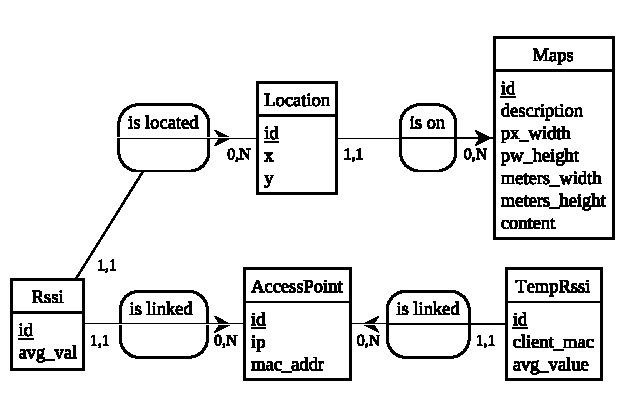
\includegraphics[scale=1]{./positioning_server/db.pdf}
  \caption{Database}
\end{figure}

        \subsection{Creation script}

\paragraph{}
In order to create the database, a postgresql script has been created. It
creates a user ``lo53'' with a password ``lo53'' and a database ``lo53\_rssi''.

        \subsection{Filling}

\paragraph{}
The filing of the database has to be handmade, except for the Maps table. As
this table contains binary data, it is quite difficult to do it manually. So we
wrote a filling script to do this. This script put maps pictures in the
database, and get informations about maps from text files like this one :

\verbatiminput{./positioning_server/pic.txt}

\paragraph{}
The size in pixel of the picture is automatically determined, thank to the PIL
library. The addition in the database uses the psycopg2 connector.

    \section{Configuration file}

\paragraph{}
Some values of the positioning server may need adjustments. These values should
not be hardcoded, because it is not practical at all. So the servlets share a
configuration file named \emph{config.properties}. Below is the content of this
file.

\verbatiminput{./positioning_server/config.properties}

\paragraph{}
This file already exists, and can be found in the WEB-INF/classes folder of the
positioning server. Without it, servlets won't be able to work correctly.

\paragraph{}
Here is the explanation for each value of this file :
\begin{description}
    \item[url, user and password] These values are used to configure database
        information.
    \item[ap\_port] It is used for the communication between servlets and access
        points. We assume that all access points use the same port.
    \item[ap\_timeout] It indicates how long must servlets wait for access points
        responses during RSSI requests.
    \item[min\_ap] It represents the minimum number of access points needed in
        order to make a RSSI request. If there is not enough router, no request
        will be made.
    \item[min\_samples] The minimum number of RSSI samples by access point
        required.
    \item[min\_measurements] The minimum number of temporary RSSI measurements
        needed in order to calculate a RSSI distance or validating the RSSI
        measurements for a location.
\end{description}
